\chapter{Datapath}

\section{R Type Instruction}

\textbf{\textit{Question}:} Draw and explain the datapath for
\red{\texttt{add \$rd, \$rs, \$rt}}
with control signals.

\textbf{\textit{Solution}:}\\
\begin{figure}[H]
   \centering
   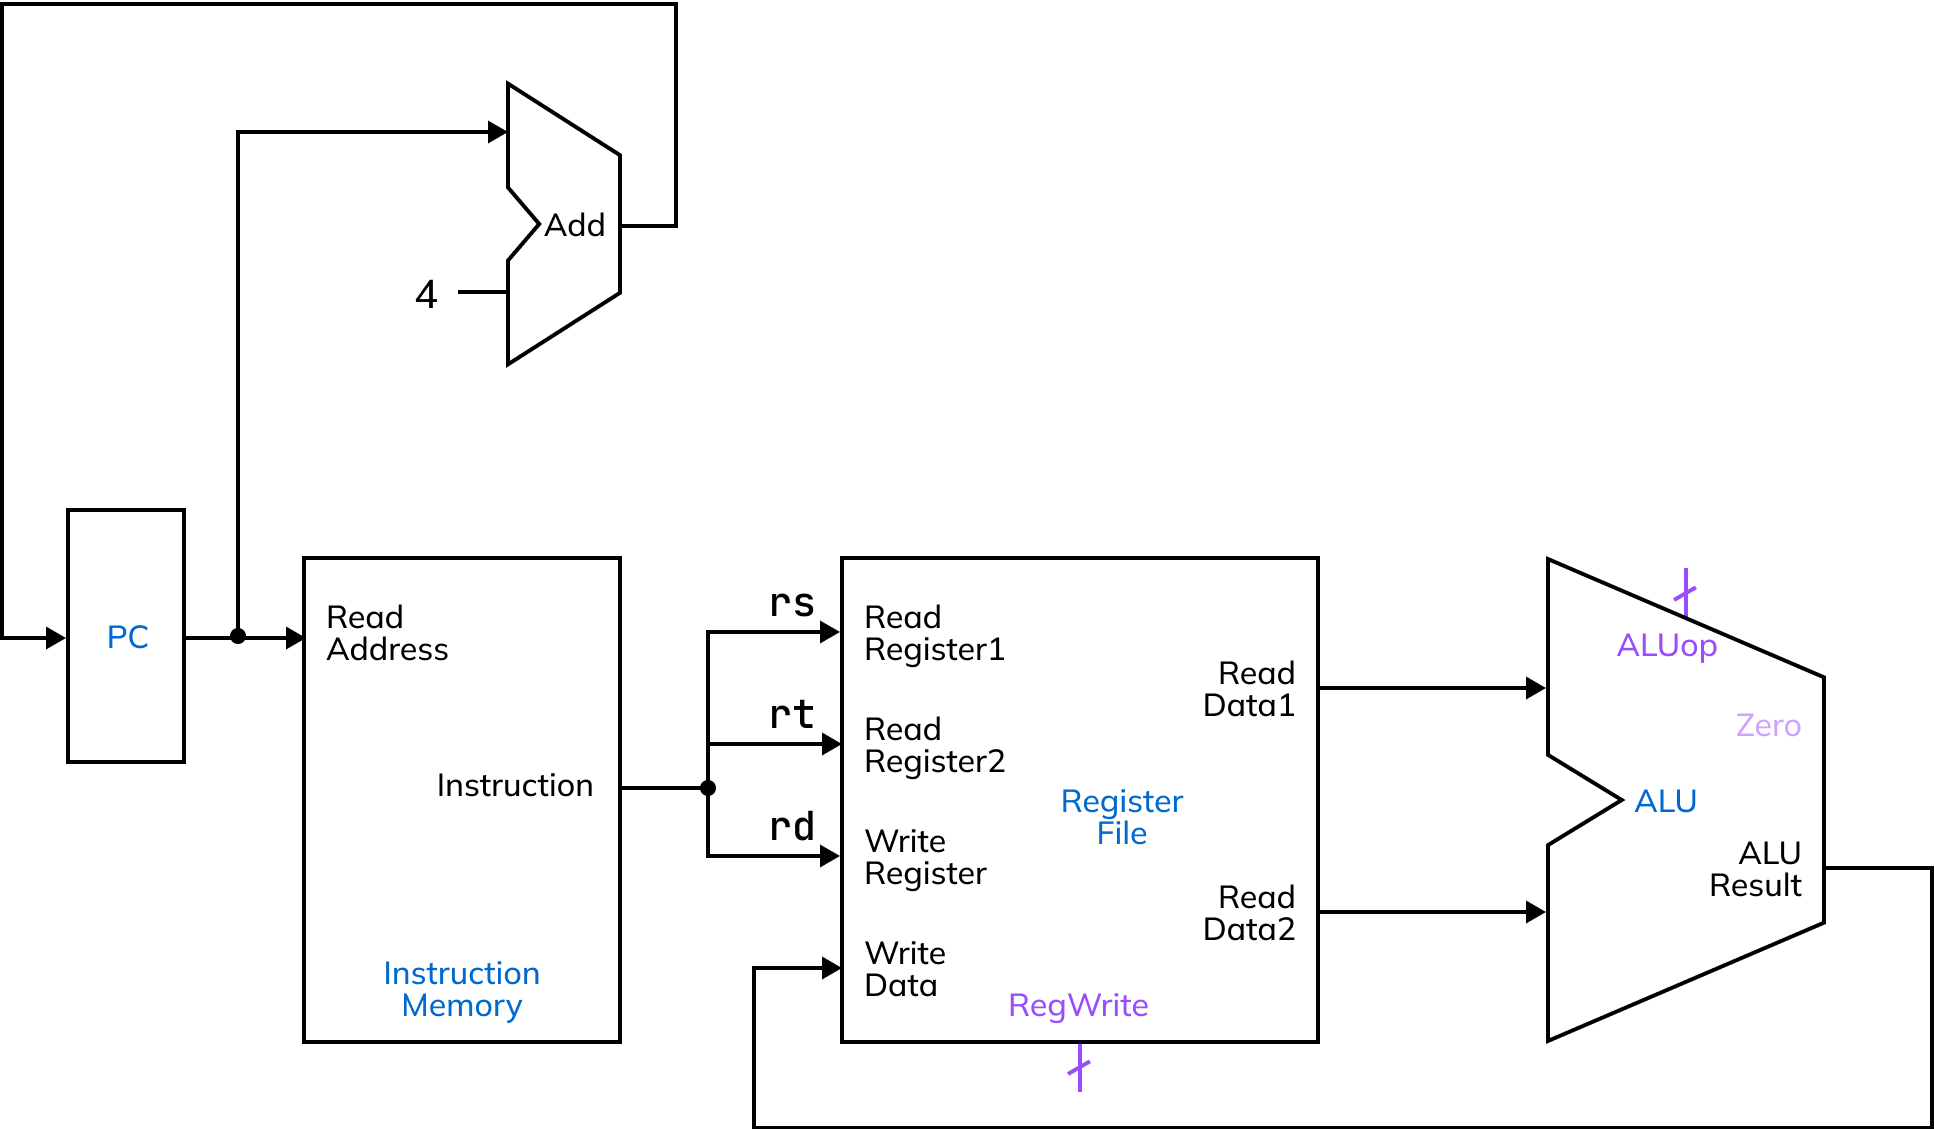
\includegraphics[width=0.65\textwidth]{figures/Datapath-ADD.png}
\end{figure}


\vspace{1em}
\begin{enumerate}
   \item Grab instruction address from PC.
   \item Fetch instruction from instruction memory.
   \item Decode instruction.
   \item Pass \rgbR{\texttt{rs}}, \rgbR{\texttt{rt}}, and \rgbR{\texttt{rd}} into read register and write register arguments.
   \item Retrieve data from \rgbO{read register 1} and \rgbO{read register 2} (\rgbR{\texttt{rs}} and \rgbR{\texttt{rt}}).
   \item Pass contents of \rgbR{\texttt{rs}} and \rgbR{\texttt{rt}} into the ALU as operands of the operation to be performed.
   \item Retrieve result of operation performed by ALU and pass back as the \rgbO{write data} argument of the register file (with the \rgbV{\texttt{RegWrite}} bit set).
   \item Add 4 bytes to the PC value to obtain the word-aligned address of the next instruction.
\end{enumerate}




\pagebreak
\section{I Type Instruction}
\subsection{Load Instruction}

\textbf{\textit{Question}:} Draw and explain the datapath for
\red{\texttt{lw \$rt, immed(\$rs)}}
with control signals.


\textbf{\textit{Solution}:}\\
\begin{figure}[H]
   \centering
   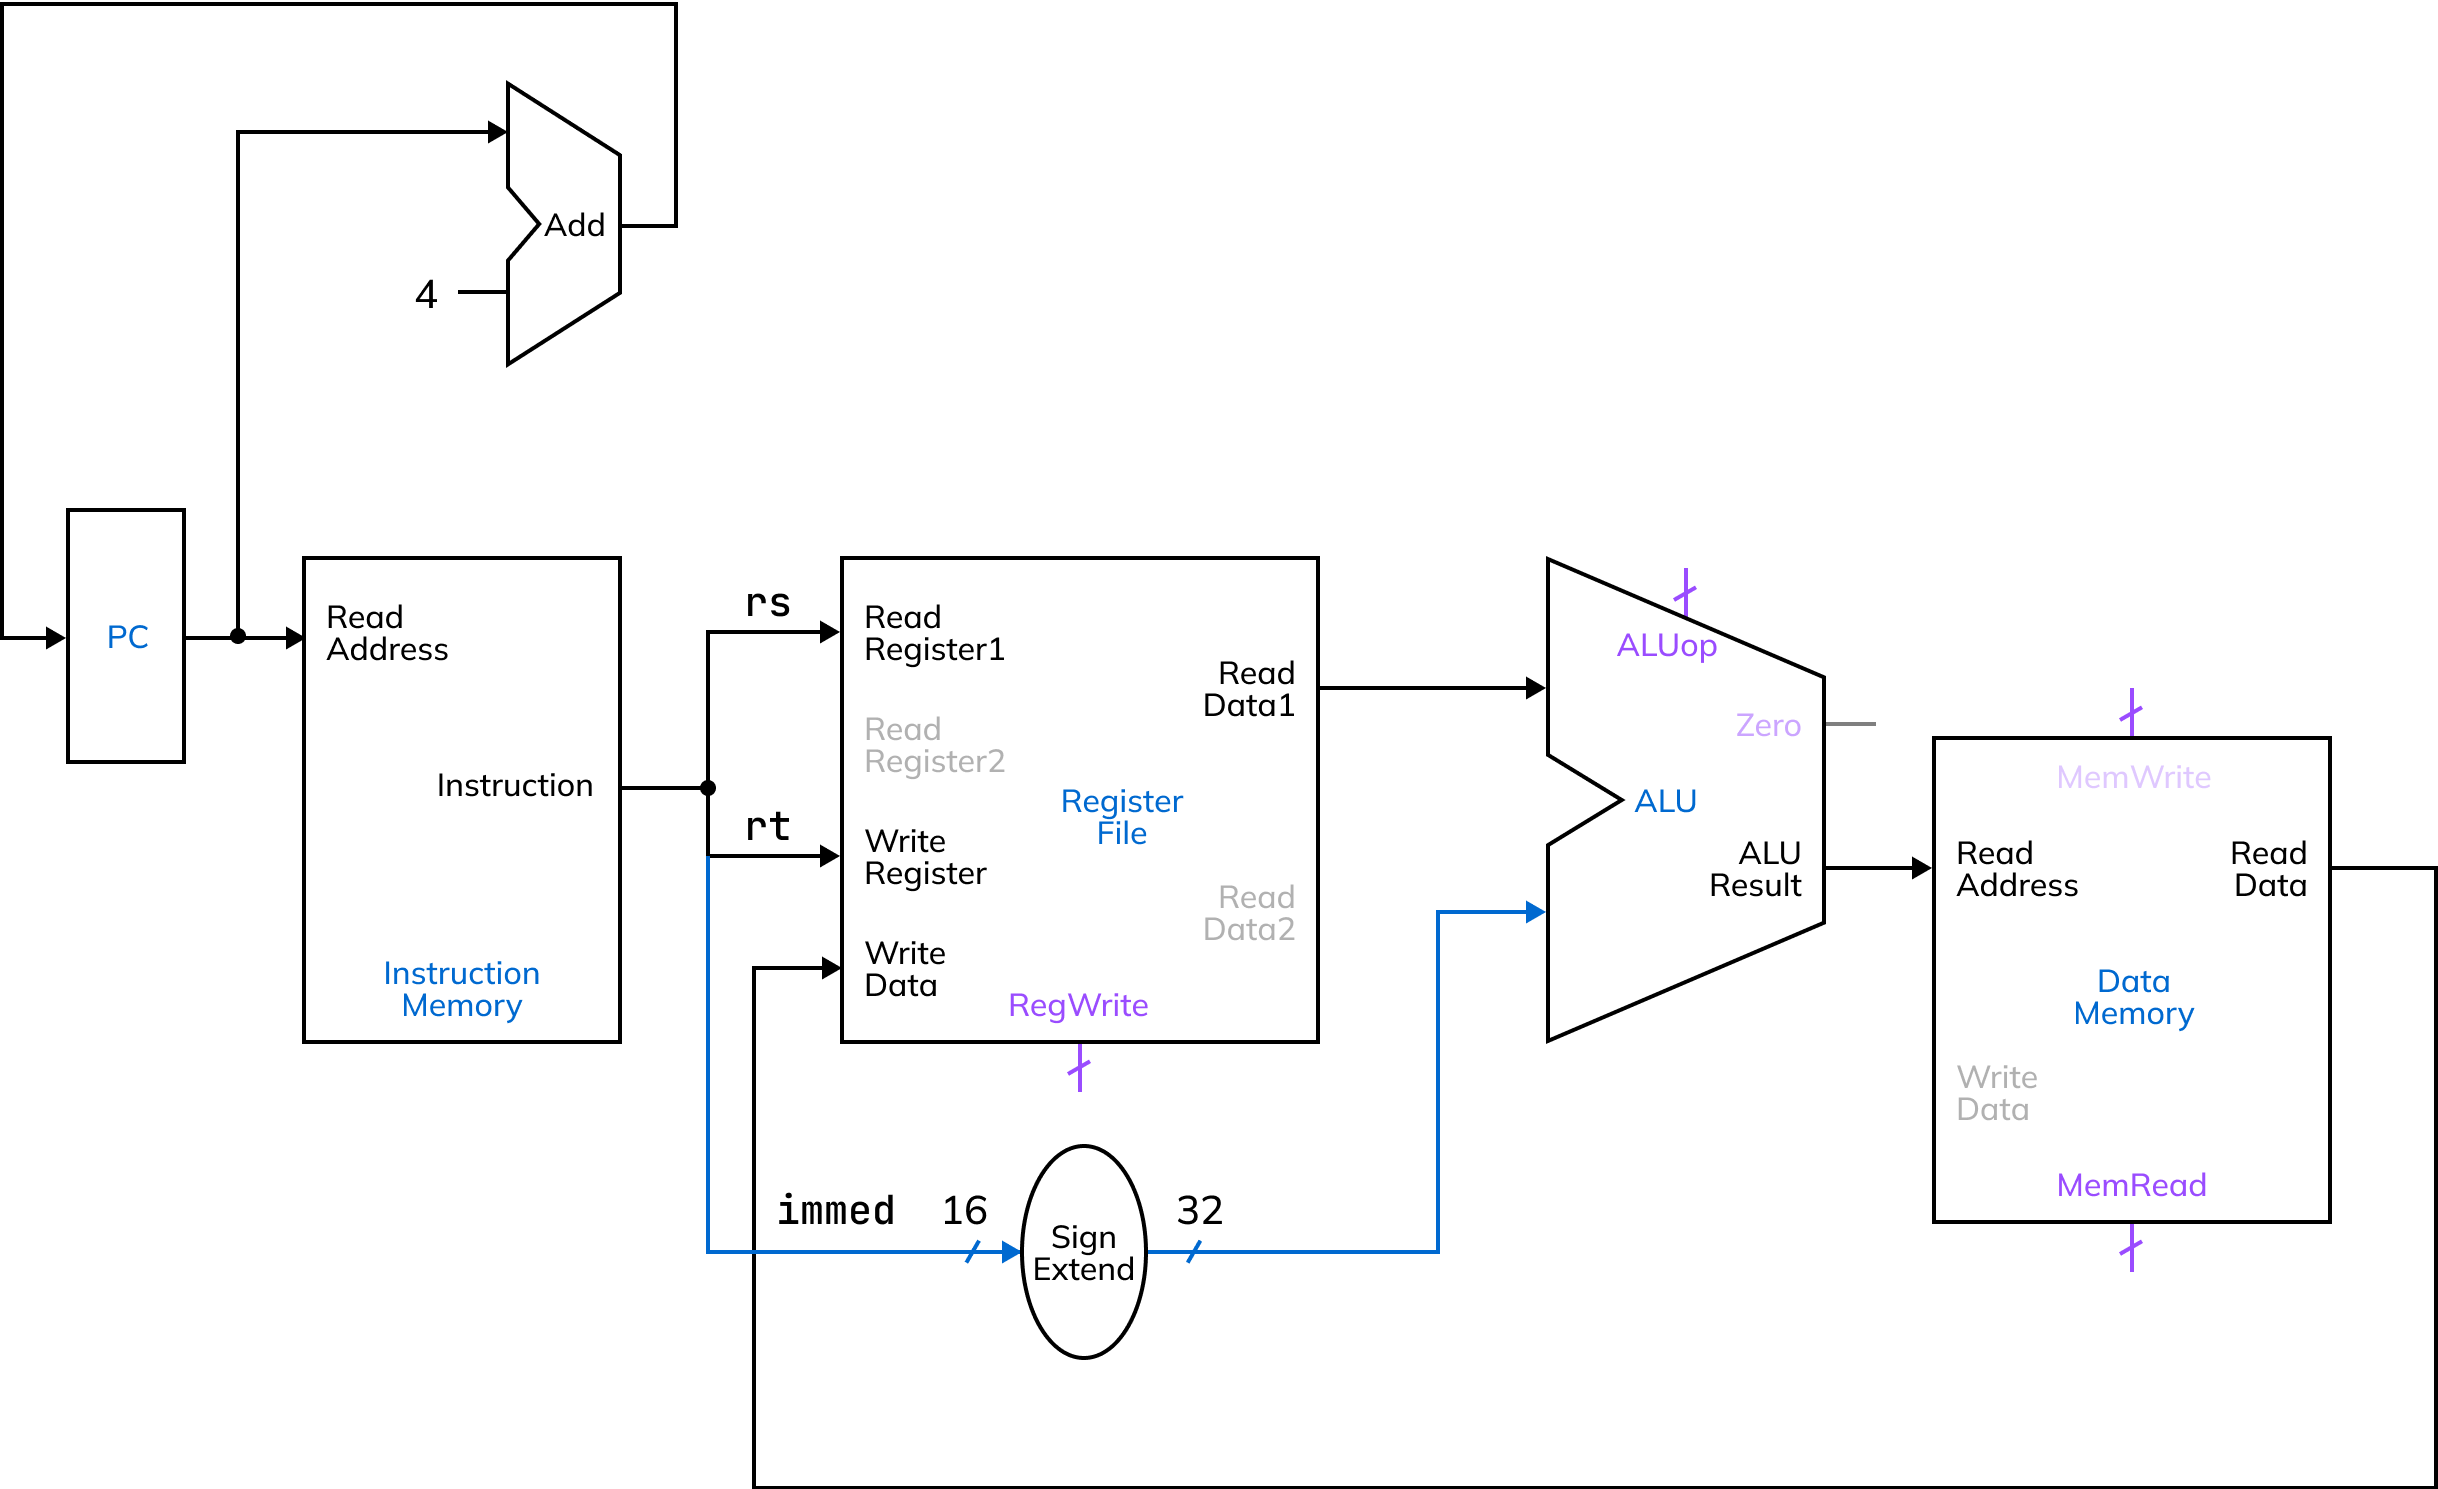
\includegraphics[width=0.75\textwidth]{figures/Datapath-LOAD.png}
\end{figure}

\vspace{1em}
\begin{enumerate}
   \item	Grab instruction address from PC.
   \item	Fetch instruction from instruction memory.
   \item	Decode instruction and extract  \rgbR{\texttt{rs}}, \rgbR{\texttt{rt}}, and \rgbR{\texttt{immediate}} fields.
   \item	Use  \rgbR{\texttt{rs}} to access base address from register file (\rgbO{read register 1}).
   \item	Sign-extend the 16-bit immediate value to 32 bits.
   \item	Add the sign-extended immediate to the value from  \rgbR{\texttt{rs}} using the ALU to calculate the address.
   \item Retrieve the calculated effective memory address from ALU and pass back as the read address argument of the data memory (with \rgbV{\texttt{MemRead}} enabled).
   \item	Retrieve the data from data memory and pass back as the \rgbO{write data} argument of the register file (with the \rgbV{\texttt{RegWrite}} bit set).
   \item	Add 4 bytes to the PC to obtain the word-aligned address of the next instruction.
\end{enumerate}



\pagebreak
\subsection{Store Instruction}

\textbf{\textit{Question}:} Draw and explain the datapath for
\red{\texttt{sw \$rt, immed(\$rs)}}
with control signals.

\textbf{\textit{Solution}:}\\
\begin{figure}[H]
   \centering
   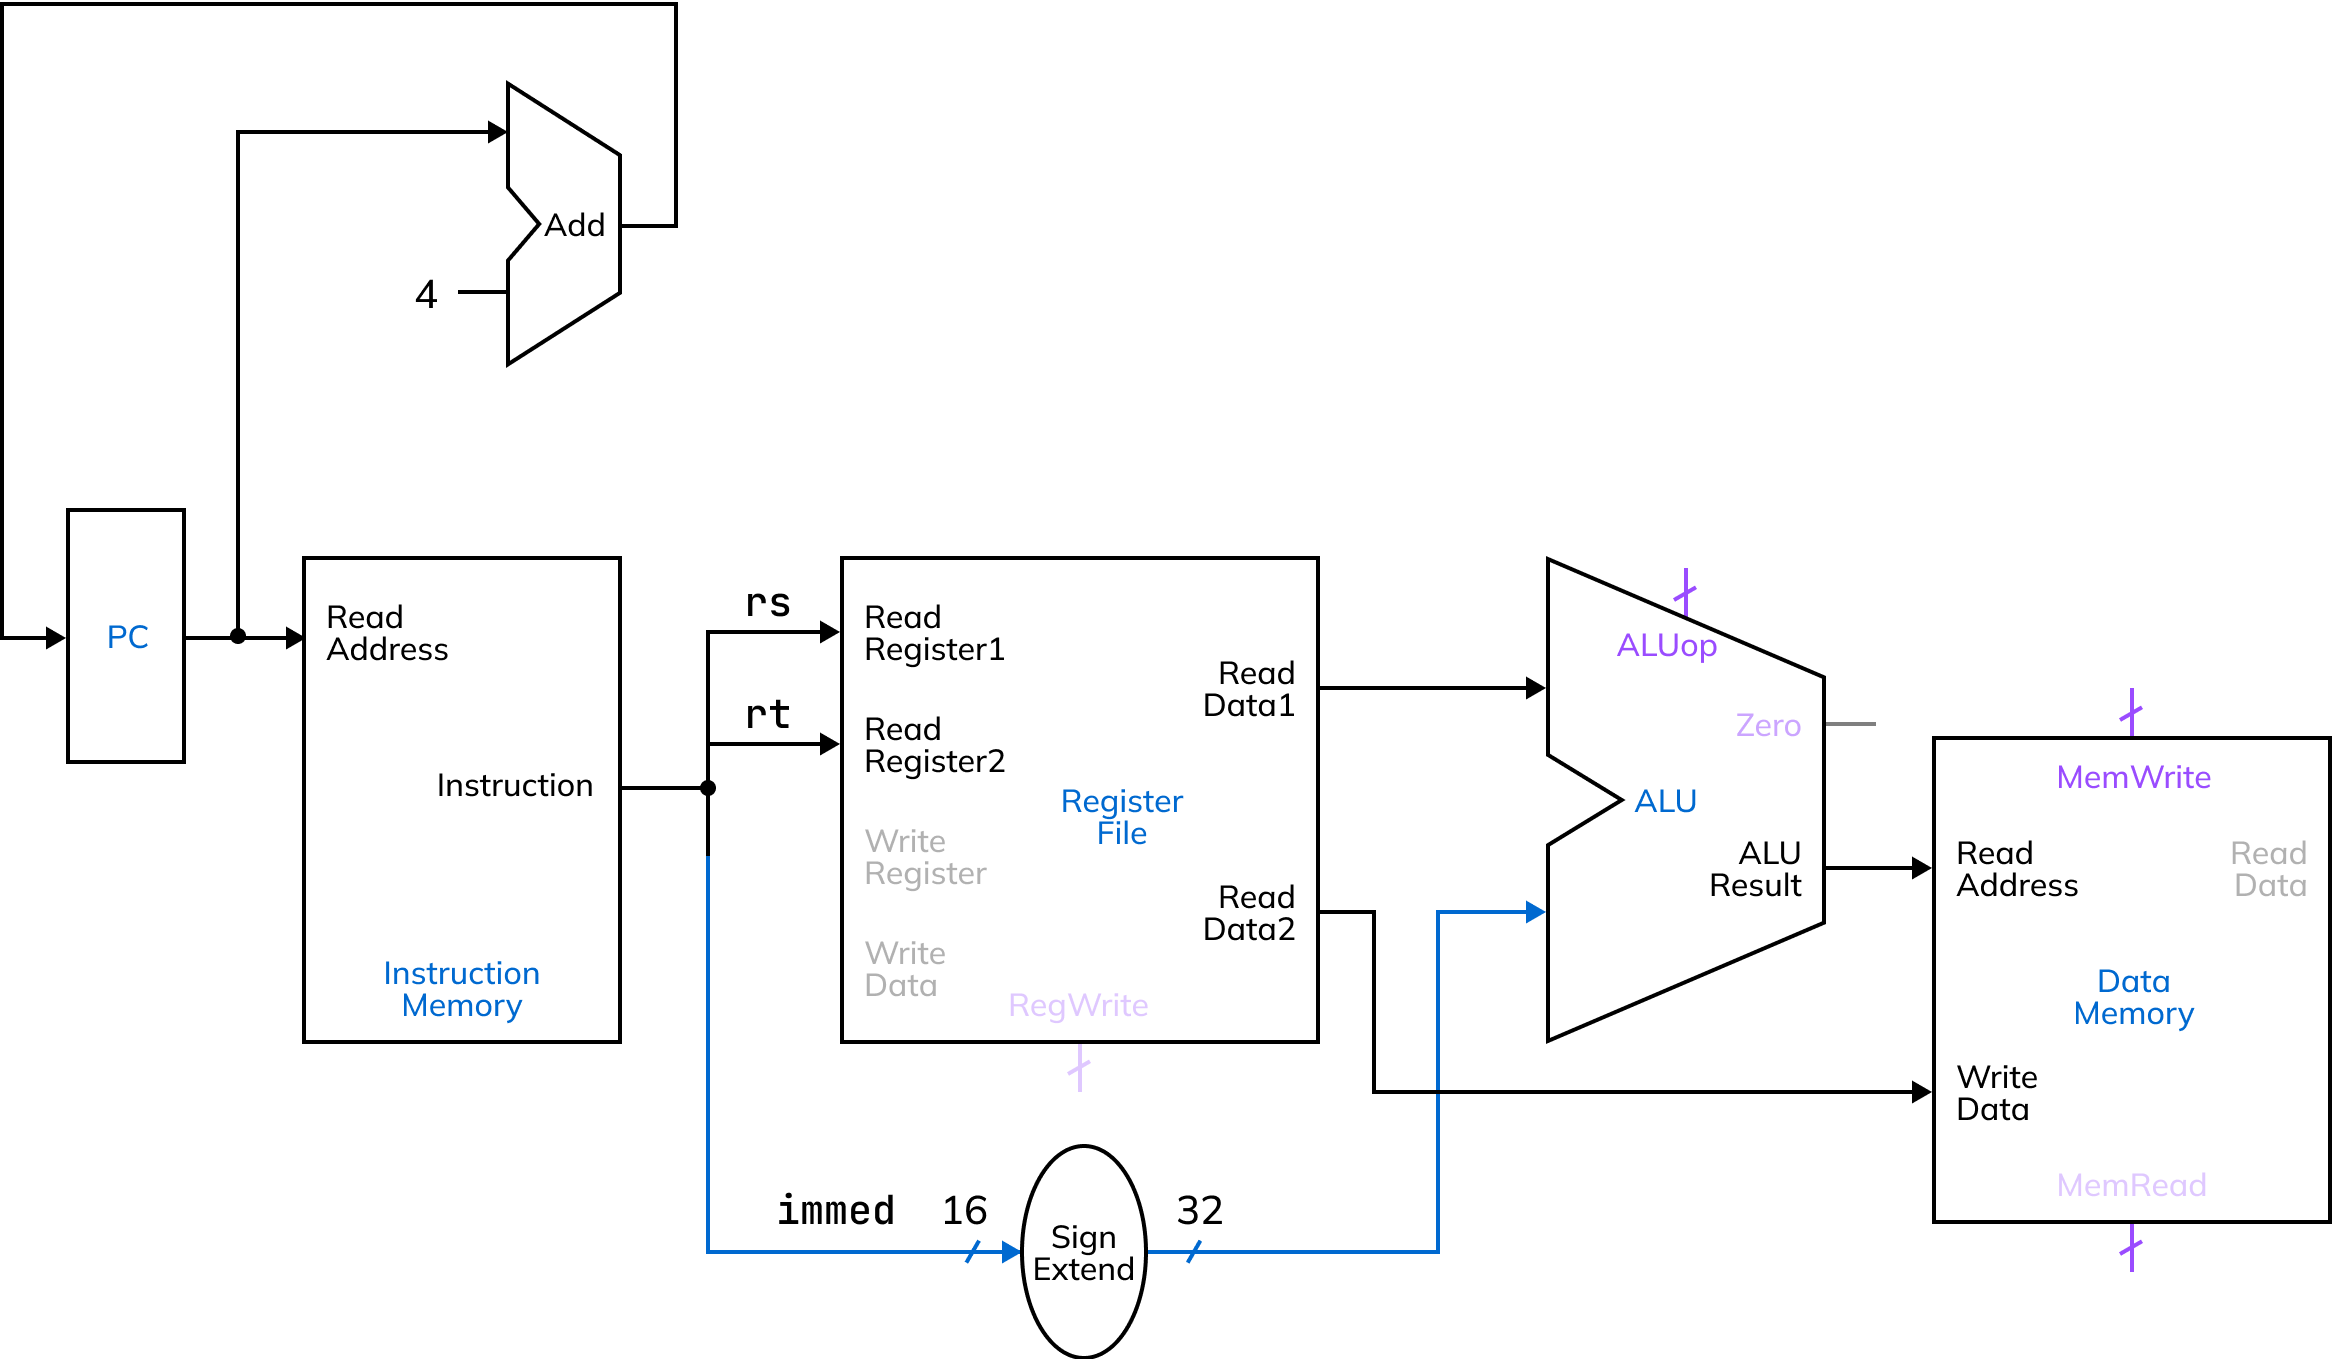
\includegraphics[width=0.75\textwidth]{figures/Datapath-STORE.png}
\end{figure}

\vspace{1em}
\begin{enumerate}
   \item	Grab instruction address from PC.
   \item	Fetch instruction from instruction memory.
   \item	Decode instruction and extract  \rgbR{\texttt{rs}}, \rgbR{\texttt{rt}}, and \rgbR{\texttt{immediate}} fields.
   \item	Use  \rgbR{\texttt{rs}} to access base address from register file (\rgbO{read register 1}).
   \item	Use  \rgbR{\texttt{rt}} to access the value that needs to be stored (\rgbO{read register 2}).
   \item	Sign-extend the 16-bit immediate value to 32 bits.
   \item	Add the sign-extended immediate to the value from  \rgbR{\texttt{rs}} using the ALU to calculate the effective memory address.
   \item Pass the ALU result as the write address to the data memory (with \rgbV{\texttt{MemWrite}} enabled).
   \item	Pass the value from \rgbR{\texttt{rt}} as the write data to memory.
   \item	Add 4 bytes to the PC to obtain the word-aligned address of the next instruction.
\end{enumerate}


\pagebreak
\subsection{Branch Instruction}

\textbf{\textit{Question}:} Draw and explain the datapath for
\red{\texttt{beq \$rs, \$rt, target}}
with control signals.

\textbf{\textit{Solution}:}\\
\begin{figure}[H]
   \centering
   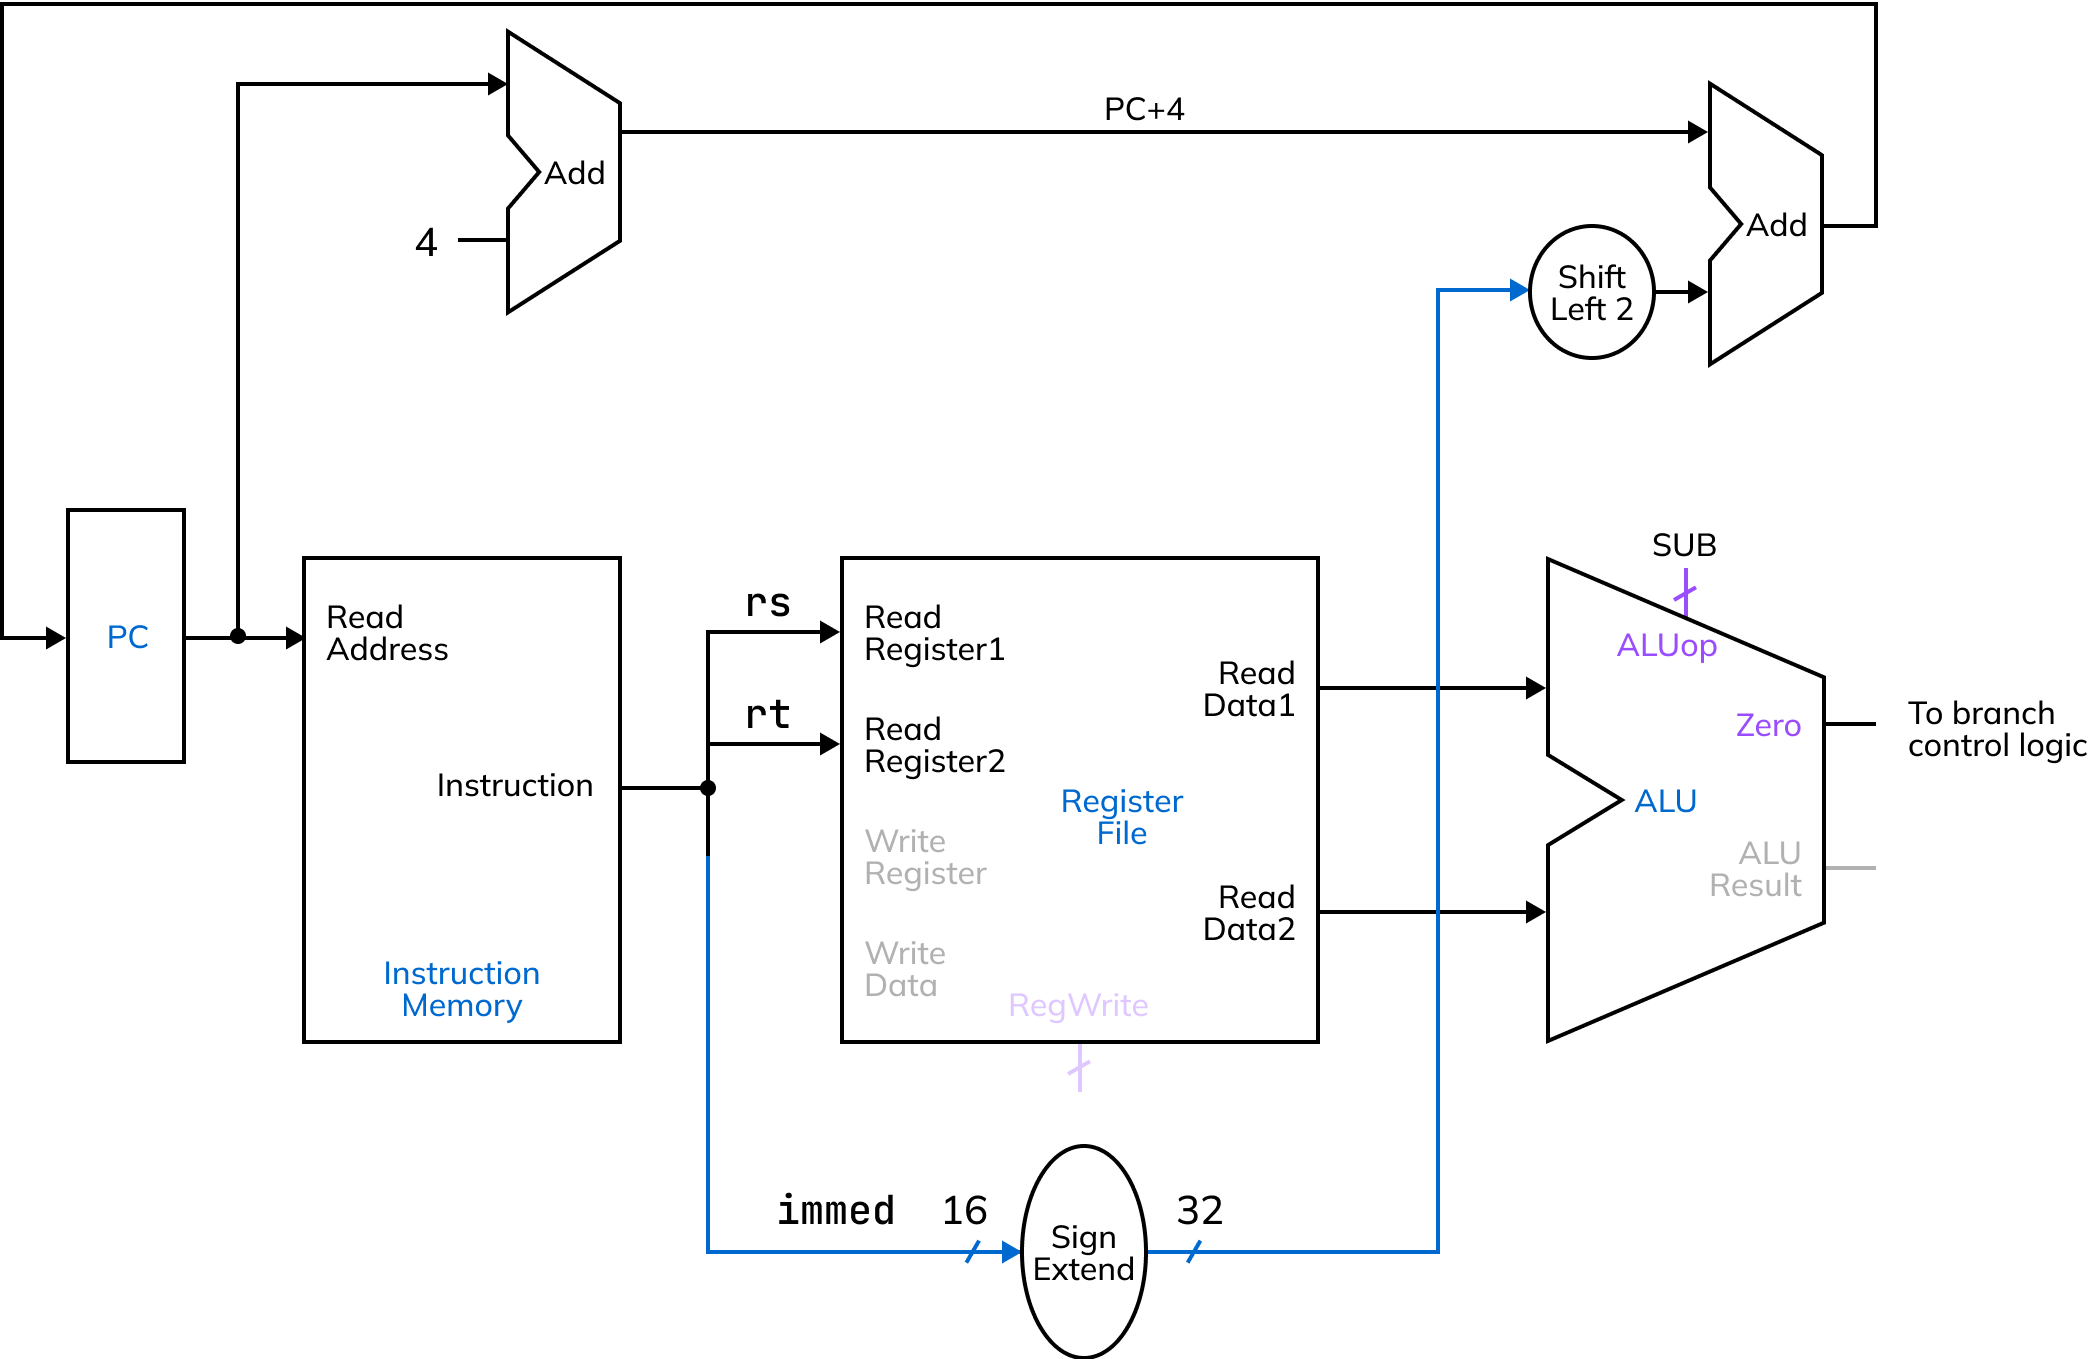
\includegraphics[width=0.75\textwidth]{figures/Datapath-BEQ.png}
\end{figure}

\vspace{1em}
\begin{enumerate}
   \item	Grab instruction address from PC.
   \item	Fetch instruction from instruction memory.
   \item	Decode instruction and extract \rgbR{\texttt{rs}}, \rgbR{\texttt{rt}}, and \rgbR{\texttt{immediate}} fields.
   \item	Use \rgbR{\texttt{rs}} and \rgbR{\texttt{rt}} to read values from register file (\rgbO{read register 1} and \rgbO{read register 2}).
   \item	Pass both register values into ALU to perform subtraction:
   \begin{itemize}
      \item ALU does: \rgbO{ReadData1} - \rgbO{ReadData2}
   \end{itemize}
   \item	Check if ALU result is zero (i.e., \rgbR{\texttt{\$t1}} = \rgbR{\texttt{\$t2}}) - set the \rgbV{\texttt{Zero}} signal.
   \item	Sign-extend the 16-bit immediate value to 32 bits.
   \item	Shift the sign-extended immediate left by 2 bits to get word-aligned offset.
   \item	Add this shifted offset to PC + 4 to calculate branch target address.
   \item	If \rgbV{\texttt{Zero}} = 1 and \rgbV{\texttt{Branch}} = 1, update PC to branch target address.
   \item	If not, PC is updated to PC + 4 to move to next instruction normally.
\end{enumerate}



\pagebreak
\section{J Type Instruction}
\subsection{Jump Instruction}

\textbf{\textit{Question}:} Draw and explain the datapath for
\red{\texttt{j target}}
with control signals.

\textbf{\textit{Solution}:}\\
\begin{figure}[H]
   \centering
   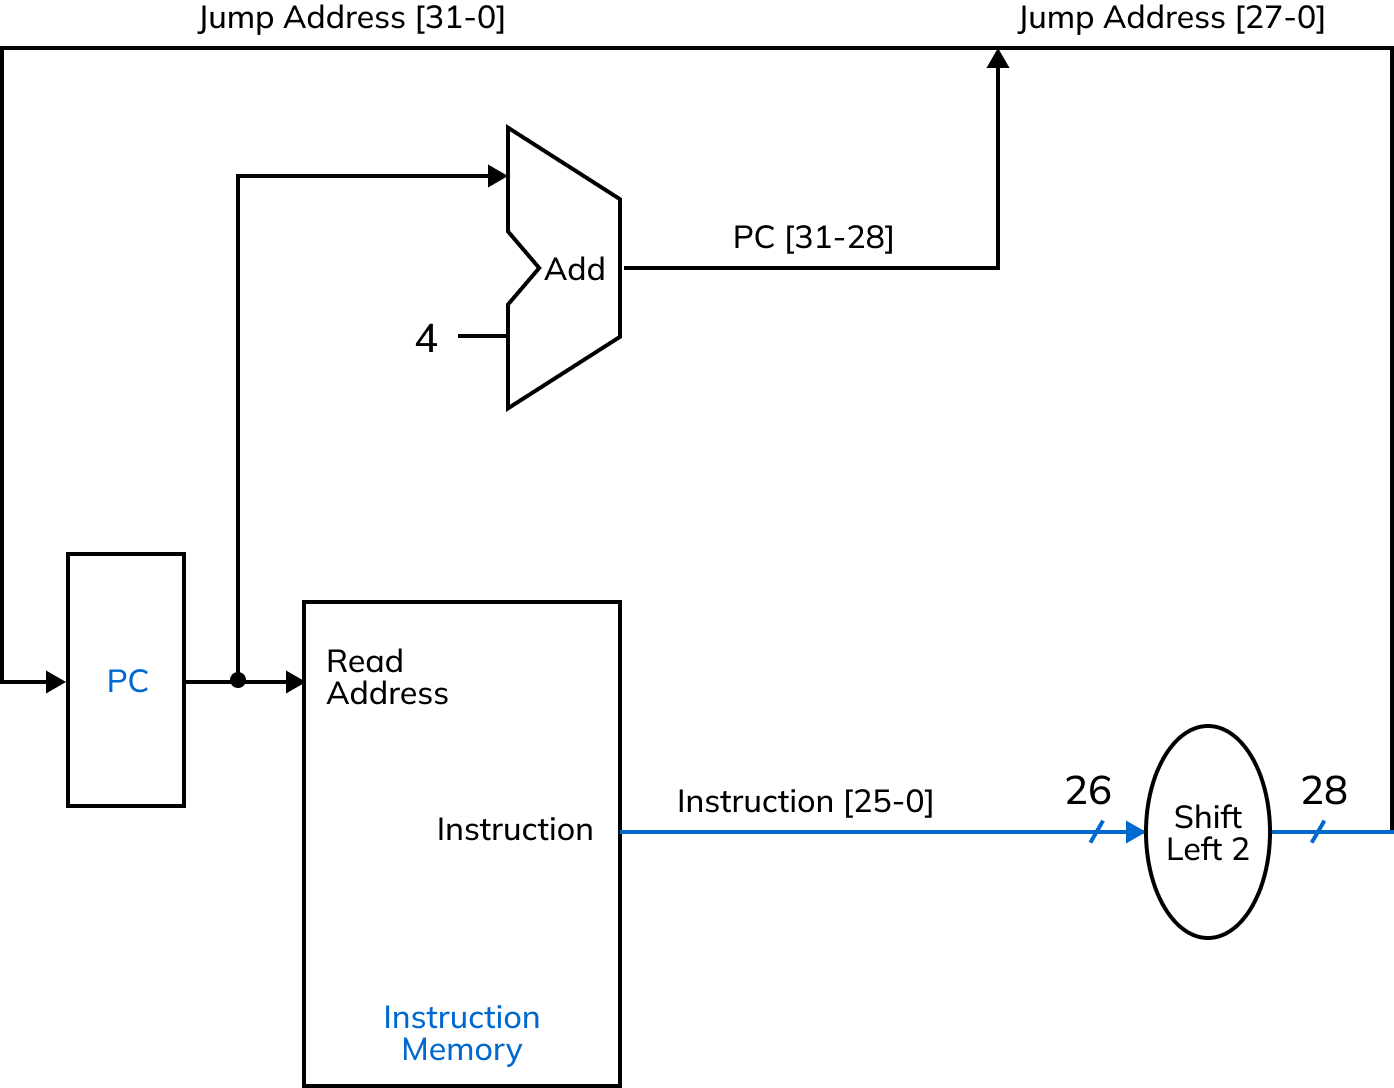
\includegraphics[width=0.55\textwidth]{figures/Datapath-JUMP.png}
\end{figure}


\vspace{1em}
\begin{enumerate}
   \item	Grab instruction address from PC.
   \item	Fetch instruction from instruction memory.
   \item	Extract the 26-bit target address field from the instruction (bits [25-0]).
   \item	Shift the 26-bit target address left by 2 bits to make it word-aligned (now 28 bits).
   \item	Take the upper 4 bits (bits [31-28]) from PC + 4 to preserve current PC region.
   \item	Concatenate upper 4 bits of PC+4 with the 28-bit shifted address → forms the full 32-bit jump address.
   \item	Load this new address into the PC → execution jumps to that address.
   \item	No register read/write or ALU operation is needed in this instruction.
\end{enumerate}